\chapter{Setup for Test of the Frequency and Time domain Response of the Effects}\label{chap:effect_test_response}

In this appendix the setup for measuring the frequency- and time- domain response of the implemented effects.

\section{Material and Setup}

The use material to perform the test is:

\begin{itemize}
	\item A computer with MATLAB, Waveforms 2015 and Code Composer
	\item Wave Generator Digilent Analog Discovery 2
	\item The \gls{dsp} TMS320C5515
	\item Wires
\end{itemize}

In \autoref{fig:appendix:dsp_frequency_response} the test setup for the measurements is shown.
The wave generator is connected to the stereo input of the DSP. Two scopes are used, one connected on the input and the other one on the output. The computer is used to load the compiled code on the DSP, inspect what is on the scopes using Waveforms 2015. 
Measuring the response in frequency domain or time domain depends on the effect, time domain may be useful in some cases and not in the others. 
 

\begin{figure}[hbt]
	\begin{picture}(0,0)%
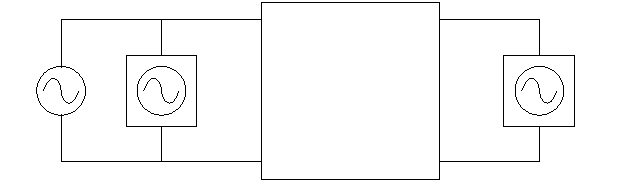
\includegraphics{overall_dsp_test.pdf}%
\end{picture}%
\setlength{\unitlength}{4144sp}%
%
\begingroup\makeatletter\ifx\SetFigFont\undefined%
\gdef\SetFigFont#1#2#3#4#5{%
  \reset@font\fontsize{#1}{#2pt}%
  \fontfamily{#3}\fontseries{#4}\fontshape{#5}%
  \selectfont}%
\fi\endgroup%
\begin{picture}(4809,1374)(-1994,152)
\put(541,749){\makebox(0,0)[lb]{\smash{{\SetFigFont{12}{14.4}{\rmdefault}{\mddefault}{\updefault}{\color[rgb]{0,0,0}DSP}%
}}}}
\put(-449,749){\makebox(0,0)[lb]{\smash{{\SetFigFont{12}{14.4}{\rmdefault}{\mddefault}{\updefault}{\color[rgb]{0,0,0}Ch1}%
}}}}
\put(2431,749){\makebox(0,0)[lb]{\smash{{\SetFigFont{12}{14.4}{\rmdefault}{\mddefault}{\updefault}{\color[rgb]{0,0,0}Ch2}%
}}}}
\put(-1979,749){\makebox(0,0)[lb]{\smash{{\SetFigFont{12}{14.4}{\rmdefault}{\mddefault}{\updefault}{\color[rgb]{0,0,0}$V_s$}%
}}}}
\end{picture}%
\caption{Figure showing the test setup}
	\label{fig:appendix:dsp_frequency_response}
\end{figure}
